%%%%%%%%%%%%%%%%%%%%%%%%%%%%%%%%%%%%%%%%%%%%%%%%%%%%%%%%%%%%%%%%%%%%%%%%%%%%%%%
% Project: GAL 2009
% Authors:
%     Radim Kapavik, xkapav01@stud.fit.vutbr.cz
%     Ondrej Lengal, xlenga00@stud.fit.vutbr.cz
%     Vojtech Storek, xstore02@stud.fit.vutbr.cz
%     Vit Triska, xtrisk01@stud.fit.vutbr.cz
%     Petr Zemek, xzemek02@stud.fit.vutbr.cz
%%%%%%%%%%%%%%%%%%%%%%%%%%%%%%%%%%%%%%%%%%%%%%%%%%%%%%%%%%%%%%%%%%%%%%%%%%%%%%%

\section*{Exercise 2}
\label{sec:Ex2}

\subsection*{Assignment}

Give an adjacency-list representation for a complete binary tree on $7$
vertices. Give an equivalent adjacency-matrix representation. Assume that
vertices are numbered from $1$ to $7$ as in a binary heap.

\subsection*{Solution}

Let $G$ be the binary tree from the assignment. Its graphical representation
can be seen in Figure~\ref{fig:Ex2-BinTree}.

\begin{figure}[h]
	\begin{center}
		\SetUpEdge[style={->}]
		\begin{tikzpicture}
			\Vertex[x=9 ,y=10]{7}
			\Vertex[x=7 ,y=9]{4}
			\Vertex[x=11,y=9]{6}
			\Vertex[x=6 ,y=8]{1}
			\Vertex[x=8 ,y=8]{3}
			\Vertex[x=10 ,y=8]{2}
			\Vertex[x=12 ,y=8]{5}
			\Edge(7)(4)
			\Edge(7)(6)
			\Edge(4)(1)
			\Edge(4)(3)
			\Edge(6)(2)
			\Edge(6)(5)
		\end{tikzpicture}
	\end{center}
	\caption{Complete binary tree $G$ on $7$ vertices.}
	\label{fig:Ex2-BinTree}
\end{figure}

Adjacency-list representation of the given binary tree can be seen in
Figure~\ref{fig:Ex2-AdjListRep}.

\begin{figure}[h]
	\begin{center}
		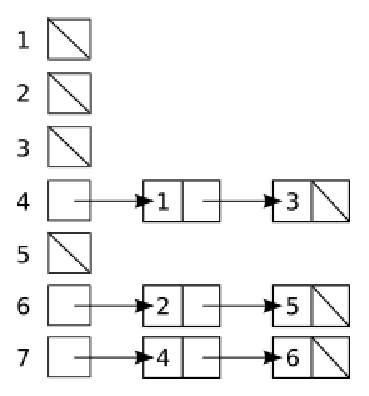
\includegraphics[width=3.5cm,keepaspectratio]{include/ex2-adj-list}
	\end{center}
	\caption{Adjacency-list representation of $G$.}
	\label{fig:Ex2-AdjListRep}
\end{figure}

Adjacency-matrix representation of the given binary tree can be seen in
Figure~\ref{fig:Ex2-AdjMatrixRep}.

\begin{figure}[h]
	\begin{center}
		\begin{tabular}{c|c c c c c c c|}
			  & 1 & 2 & 3 & 4 & 5 & 6 & 7 \\
			\hline
			1 & 0 & 0 & 0 & 0 & 0 & 0 & 0 \\
			2 & 0 & 0 & 0 & 0 & 0 & 0 & 0 \\
			3 & 0 & 0 & 0 & 0 & 0 & 0 & 0 \\
			4 & 1 & 0 & 1 & 0 & 0 & 0 & 0 \\
			5 & 0 & 0 & 0 & 0 & 0 & 0 & 0 \\
			6 & 0 & 1 & 0 & 0 & 1 & 0 & 0 \\
			7 & 0 & 0 & 0 & 1 & 0 & 1 & 0 \\
			8 & 0 & 0 & 0 & 0 & 0 & 0 & 0 \\
			\hline
		\end{tabular}
	\end{center}
	\caption{Adjacency-matrix representation of $G$.}
	\label{fig:Ex2-AdjMatrixRep}
\end{figure}

%%%%%%%%%%%%%%%%%%%%%%%%%%%%%%%%%%%%%%%%%%%%%%%%%%%%%%%%%%%%%%%%%%%%%%%%%%%%%%%
% vim: syntax=tex
%%%%%%%%%%%%%%%%%%%%%%%%%%%%%%%%%%%%%%%%%%%%%%%%%%%%%%%%%%%%%%%%%%%%%%%%%%%%%%%
